
%% Harvard Physics Project
%% Test Booklet 4: Light and Electromagnetism
%%--------------------------------------------------


%% Test Booklet 4 contains 70 - 2 questions


%% Test A
%%--------------------
\element{project}{
\begin{question}{testA-Q01}
    A person whose eyes are located at point $P$ is looking into the mirror.
    \begin{center}
    \begin{tikzpicture}
        %% mirror
        \draw[line width=1pt] (-0.15,0) -- (2.15,0) node[pos=0.5,anchor=south] {mirror};
        %% point P
        \draw[fill] (-1.5,-0.5) circle (1.5pt) node[anchor=east] {$P$};
        %% cards 1,2,3,4
        \node[draw,minimum height=1.5em,minimum width=0.5em,anchor=north] at (0,-0.25) {1};
        \node[draw,minimum height=1.5em,minimum width=0.5em,anchor=north] at (2,-0.25) {2};
        \node[draw,minimum height=1.5em,minimum width=0.5em,anchor=north] at (1,-2) {4};
        \node[draw,minimum height=1.5em,minimum width=0.5em,anchor=north] at (4,-0.25) {3};
    \end{tikzpicture}
    \end{center}
    Which of the numbered cards can he see reflected in the mirror?
    \begin{multicols}{2}
    \begin{choices}
        %% NOTE: questionmult??
        %\wrongchoice{1}
        %\wrongchoice{2}
        %\wrongchoice{3}
        %\wrongchoice{4}
        \wrongchoice{1 and 4}
      \correctchoice{2 and 3}
        \wrongchoice{1, 2 and 3}
        \wrongchoice{1, 2, 3 and 4}
    \end{choices}
    \end{multicols}
\end{question}
}

\element{project}{
\begin{question}{testA-Q02}
    A point charge $+Q_1$ exerts an electrostatic force $F$
        on point charge $+Q_2$ \SI{3}{\centi\meter} away.
    If the charges are placed \SI{6}{\centi\meter} apart,
        the magnitude of the electrostatic force $+Q_1$ exerts on $+Q_2$ will be:
    \begin{multicols}{3}
    \begin{choices}
        \wrongchoice{$4F$}
        \wrongchoice{$2F$}
        \wrongchoice{$F$}
        \wrongchoice{$\dfrac{F}{2}$}
      \correctchoice{$\dfrac{F}{4}$}
    \end{choices}
    \end{multicols}
\end{question}
}

\element{project}{
\begin{question}{testA-Q03}
    A narrow beam of light emerges from a block of ordinary glass
        in the direction shown in the diagram.
    \begin{center}
    \begin{tikzpicture}
        %% NOTE: used n=1.50 for glass
        %% glass
        \draw[white,fill=white!90!black] (0,-2) arc(270:90:2) -- cycle;
        %% surface
        \draw[line width=1pt] (0,-2.1) -- (0,2.1);
        %% incoming
        \foreach \a/\b in {120/A,135/B,150/C,180/D,200/E} {
            \draw[thick,postaction={decorate},decoration={markings, mark=at position 0.5 with {\arrow{latex}}}] (\a:2.33) -- (0,0) node[pos=0,anchor=center,shift={(\a:1em)}] {$\b$};
        }
        %% outgoing
        \draw[thick,->] (0,0) -- (315:2);
        %% labels
        \node[anchor=north] at (-0.8,-2.2) {glass};
        \node[anchor=north] at (+0.8,-2.2) {air};
    \end{tikzpicture}
    \end{center}
    Which arrow in the diagram best represents the path
        of the beam within the glass?
    \begin{multicols}{5}
    \begin{choices}[o]
        \wrongchoice{$A$}
        \wrongchoice{$B$}
      \correctchoice{$C$}
        \wrongchoice{$D$}
        \wrongchoice{$E$}
    \end{choices}
    \end{multicols}
\end{question}
}

\element{project}{
\begin{question}{testA-Q04}
    Two spheres, $A$ and $B$, are \SI{4}{\meter} apart.
    A charge of $2Q$ is distributed over sphere $A$
        and a charge of $Q$ is distributed over sphere $B$.
    (See sketch.)
    \begin{center}
    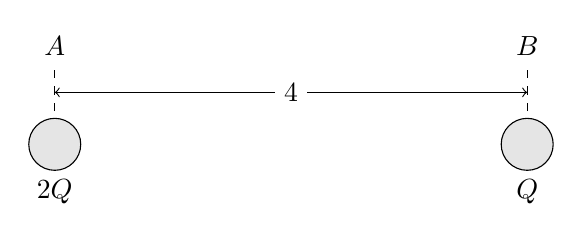
\begin{tikzpicture}
        %% sphere A
        \draw[dashed] (-3,0) -- ++(90:1) node[anchor=south] {$A$};
        \draw[fill=white!90!black] (-3,0) circle (0.33);
        \node[anchor=north] at (-3,-0.33) {$2Q$};
        %% sphere B
        \draw[dashed] (+3,0) -- ++(90:1) node[anchor=south] {$B$};
        \draw[fill=white!90!black] (+3,0) circle (0.33);
        \node[anchor=north] at (+3,-0.33) {$Q$};
        %% 4 meter
        \draw[<->] (-3,0.66) -- (3,0.66) node[pos=0.5,anchor=center,fill=white] {\SI{4}{\meter}};
    \end{tikzpicture}
    \end{center}
    How does the magnitude of the force exerted by $A$ on $B$
        compare with the magnitude of the force exerted by $B$ on $A$?
    \begin{choices}
        \wrongchoice{The force on $A$ is 4 times the force on $B$.}
        \wrongchoice{The force on $A$ is 2 times the force on $B$.}
      \correctchoice{The force on $A$ is the same as the force on $B$.}
        \wrongchoice{The force on $A$ is $\dfrac{1}{2}$ the force on $B$.}
        \wrongchoice{The force on $A$ is $\dfrac{1}{4}$ the force on $B$.}
    \end{choices}
\end{question}
}

\element{project}{
\begin{question}{testA-Q05}
    Which of the arrows indicates the direction of the electric field
        at point $P$ due to the stationary charges $+Q$ and $-Q$?
    \begin{center}
    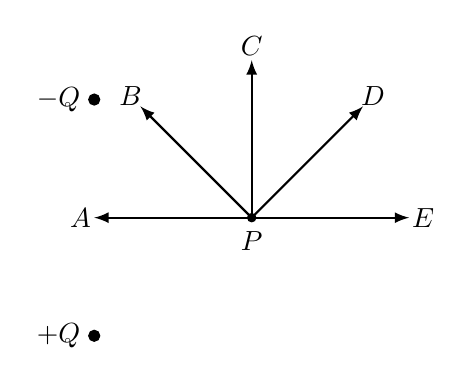
\begin{tikzpicture}
        %% Point P
        \draw[fill] (0,0) circle (1.5pt) node[anchor=north,yshift=-1.5pt] {$P$};
        %% Vector A,B,C,D,E
        \foreach \a/\b in {180/A, 135/B, 90/C, 45/D, 0/E} {
            \draw[thick,-latex] (0,0) -- (\a:2) node[anchor=center,shift={(\a:0.5em)}] {$\b$};
        }
        %% Charges +Q and -Q
        \draw[fill] (-2,+1.5) circle (2pt) node[anchor=east,xshift=-1.5pt] {$-Q$};
        \draw[fill] (-2,-1.5) circle (2pt) node[anchor=east,xshift=-1.5pt] {$+Q$};
    \end{tikzpicture}
    \end{center}
    \begin{multicols}{5}
    \begin{choices}[o]
        %% NOTE: move tikz to options?
        \wrongchoice{$A$}
        \wrongchoice{$B$}
      \correctchoice{$C$}
        \wrongchoice{$D$}
        \wrongchoice{$E$}
    \end{choices}
    \end{multicols}
\end{question}
}

\element{project}{
\begin{question}{testA-Q06}
    The first definite evidence that light moves at a finite speed was found by:
    \begin{choices}
        \wrongchoice{Galileo Galilei.}
      \correctchoice{Ole Christensen R{\o}mer.}
        \wrongchoice{Christiaan Huygens}
        \wrongchoice{Thomas Young.}
    \end{choices}
\end{question}
}

\element{project}{
\begin{question}{testA-Q07}
    In a vacuum, electromagnetic radiations such as radio waves,
        light, x-rays and gamma rays have the same:
    \begin{multicols}{2}
    \begin{choices}
        \wrongchoice{wave length.}
        \wrongchoice{frequency.}
        \wrongchoice{period.}
      \correctchoice{speed.}
        \wrongchoice{amplitude.}
    \end{choices}
    \end{multicols}
\end{question}
}

\element{project}{
\begin{question}{testA-Q08}
    Newton's synthesis of terrestrial and celestial mechanics
        incorporated the work of Kepler and Galileo.
    In a similar way, the work of {\o}rsted and Faraday
        was incorporated in the synthesis made by:
    %Hans Christian Ørsted
    %Michael Faraday
    \begin{choices}
        \wrongchoice{Andr\'{e}-Marie Amp\`{e}re.}
        \wrongchoice{Heinrich Rudolf Hertz.}
      \correctchoice{James Clerk Maxwell.}
        \wrongchoice{William Gilbert.}
    \end{choices}
\end{question}
}

\element{project}{
\begin{questionmult}{testA-Q09}
    The direction of the electric field in a plane electromagnetic wave is:
    %% NOTE: questionmult if three options
    \begin{choices}
        \wrongchoice{perpendicular to the magnetic field and in the direction of the wave's propagation.}
      \correctchoice{perpendicular to the magnetic field and perpendicular to the direction of the wave's propagation.}
        \wrongchoice{parallel to the magnetic field.}
    \end{choices}
\end{questionmult}
}

\element{project}{
\begin{question}{testA-Q10}
    Power is:
    \begin{choices}
        \wrongchoice{work.}
        \wrongchoice{electrical current.}
        \wrongchoice{the rate of flow of electric charge.}
      \correctchoice{the rate of doing work.}
    \end{choices}
\end{question}
}

\element{project}{
\begin{question}{testA-Q11}
    A transformer changes:
    \begin{choices}
        \wrongchoice{electrical energy into mechanical energy,}
        \wrongchoice{mechanical energy into electrical energy.}
        \wrongchoice{high voltage dc to low voltage dc.}
      \correctchoice{low voltage ac to high voltage ac.}
    \end{choices}
\end{question}
}

\element{project}{
\begin{question}{testA-Q12}
    An example of electromagnetic induction is the:
    \begin{choices}
        \wrongchoice{magnetic field about a conductor carrying a current.}
        \wrongchoice{force between a magnet and a wire carrying a current.}
      \correctchoice{production of a current in a wire owing to a changing magnetic field.}
        \wrongchoice{force between two wires carrying electric currents.}
        \wrongchoice{depositing of an element at the cathode of an electrolytic cell.}
    \end{choices}
\end{question}
}

\element{project}{
\begin{question}{testA-Q13}
    Select the statement that best describes the scientific contribution of
        James Clerk Maxwell.
    \begin{choices}
        \wrongchoice{Two current-carrying wires exert forces on each other.}
      \correctchoice{An electric field changing with time generates a magnetic field.}
        \wrongchoice{An electric current exerts a force on a magnet.}
        \wrongchoice{A magnetic field changing with time can cause a current to flow in a wire.}
    \end{choices}
\end{question}
}

\element{project}{
\begin{question}{testA-Q14}
    %Questions 13, 14 and 15 list the names of scientists who made significant contributions to the study of electromagnetic phenomena.
    %Select the statement that best describes a contribution of each of the scientists.
    Select the statement that best describes the scientific contribution of
        Andr\'{e}-Marie Amp\`{e}re.
    \begin{choices}
      \correctchoice{Two current-carrying wires exert forces on each other.}
        \wrongchoice{An electric field changing with time generates a magnetic field.}
        \wrongchoice{An electric current exerts a force on a magnet.}
        \wrongchoice{A magnetic field changing with time can cause a current to flow in a wire.}
    \end{choices}
\end{question}
}

\element{project}{
\begin{question}{testA-Q15}
    Select the statement that best describes the scientific contribution of
        Michael Faraday.
    \begin{choices}
        \wrongchoice{Two current-carrying wires exert forces on each other.}
        \wrongchoice{An electric field changing with time generates a magnetic field.}
        \wrongchoice{An electric current exerts a force on a magnet.}
      \correctchoice{A magnetic field changing with time can cause a current to flow in a wire.}
    \end{choices}
\end{question}
}


%% Test B
%%--------------------
\element{project}{
\begin{question}{testB-Q01}
    Which of the following graphs best represents the way the
        force one small charged body exerts on another changes
        when the distance between their centers is changed?
    \begin{multicols}{2}
    \begin{choices}
        \AMCboxDimensions{down=-2.5em}
        \wrongchoice{
            \begin{tikzpicture}
                \begin{axis}[
                    axis y line=left,
                    axis x line=bottom,
                    axis line style={->},
                    xlabel={distance},
                    xtick=\empty,
                    ylabel={force},
                    ytick=\empty,
                    xmin=0,xmax=11,
                    ymin=0,ymax=11,
                    width=1.00\columnwidth,
                    very thin,
                ]
                \addplot[line width=1pt,domain=0:10]{8};
                \end{axis}
            \end{tikzpicture}
        }
        \wrongchoice{
            \begin{tikzpicture}
                \begin{axis}[
                    axis y line=left,
                    axis x line=bottom,
                    axis line style={->},
                    xlabel={distance},
                    xtick=\empty,
                    ylabel={force},
                    ytick=\empty,
                    xmin=0,xmax=11,
                    ymin=0,ymax=11,
                    width=1.00\columnwidth,
                    very thin,
                ]
                \addplot[line width=1pt,domain=0:10]{x};
                \end{axis}
            \end{tikzpicture}
        }
        \wrongchoice{
            \begin{tikzpicture}
                \begin{axis}[
                    axis y line=left,
                    axis x line=bottom,
                    axis line style={->},
                    xlabel={distance},
                    xtick=\empty,
                    ylabel={force},
                    ytick=\empty,
                    xmin=0,xmax=11,
                    ymin=0,ymax=11,
                    width=1.00\columnwidth,
                    very thin,
                ]
                \addplot[line width=1pt,domain=0:10]{10-x};
                \end{axis}
            \end{tikzpicture}
        }
        \wrongchoice{
            \begin{tikzpicture}
                \begin{axis}[
                    axis y line=left,
                    axis x line=bottom,
                    axis line style={->},
                    xlabel={distance},
                    xtick=\empty,
                    ylabel={force},
                    ytick=\empty,
                    xmin=0,xmax=11,
                    ymin=0,ymax=11,
                    width=1.00\columnwidth,
                    very thin,
                ]
                \addplot[line width=1pt,domain=0:10]{0.1*x*x};
                \end{axis}
            \end{tikzpicture}
        }
        %% NOTE: F = gmm/R^2
        %% NOTE: should be 10/x/x, but this is easier to see
        \correctchoice{
            \begin{tikzpicture}
                \begin{axis}[
                    axis y line=left,
                    axis x line=bottom,
                    axis line style={->},
                    xlabel={distance},
                    xtick=\empty,
                    ylabel={force},
                    ytick=\empty,
                    xmin=0,xmax=11,
                    ymin=0,ymax=11,
                    width=1.00\columnwidth,
                    very thin,
                ]
                \addplot[line width=1pt,domain=0:10]{10/x};
                \end{axis}
            \end{tikzpicture}
        }
    \end{choices}
    \end{multicols}
\end{question}
}

\element{project}{
\begin{question}{testB-Q02}
    \emph{All except one} of the following satisfy the
        definition of a field as given in the text.
    Find the exception.
    \begin{choices}
        \wrongchoice{water temperature in Lake Michigan}
        \wrongchoice{density of smoke in the air above New York}
        \wrongchoice{noise level in a stadium during a baseball game}
        \wrongchoice{depth of snow on the ground during a blizzard}
      \correctchoice{the total number of babies born in the United States during 1965}
    \end{choices}
\end{question}
}

\element{project}{
\begin{question}{testB-Q03}
    Which of the following is not an electromagnetic wave phenomenon?
    \begin{choices}
        \wrongchoice{radar}
        \wrongchoice{ultraviolet light}
      \correctchoice{sound}
        \wrongchoice{x-radiation}
    \end{choices}
\end{question}
}

\element{project}{
\begin{question}{testB-Q04}
    A coulomb (\si{\coulomb}) is a unit of:
    \begin{choices}
        \wrongchoice{resistance.}
        \wrongchoice{power.}
        \wrongchoice{current.}
        \wrongchoice{potential difference.}
      \correctchoice{charge.}
    \end{choices}
\end{question}
}

\element{project}{
\begin{question}{testB-Q05}
    %Questions 5, 6 and 7 list the names of scientists who made
    %    significant contributions in the study of light.
    Select the statement from the list below that best describes
        the scientific contribution of Thomas Young.
    \begin{choices}
      \correctchoice{showed that light exhibits the phenomenon of interference}
        \wrongchoice{found that color is not an inherent property of an object,
            but depends on how the object reflects and absorbs the various colored rays that strike it}
        \wrongchoice{invented a plastic sheet that would polarize light}
        \wrongchoice{developed a mathematical wave theory of light}
    \end{choices}
\end{question}
}

\element{project}{
\begin{question}{testB-Q06}
    Select the statement from the list below that best describes
        the scientific contribution of Augustin-Jean Fresnel.
    \begin{choices}
        \wrongchoice{showed that light exhibits the phenomenon of interference}
        \wrongchoice{found that color is not an inherent property of an object,
            but depends on how the object reflects and absorbs the various colored rays that strike it}
        \wrongchoice{invented a plastic sheet that would polarize light}
      \correctchoice{developed a mathematical wave theory of light}
    \end{choices}
\end{question}
}

\element{project}{
\begin{question}{testB-Q07}
    Select the statement from the list below that best describes
        the scientific contribution of Isaac Newton.
    \begin{choices}
        \wrongchoice{showed that light exhibits the phenomenon of interference}
      \correctchoice{found that color is not an inherent property of an object,
            but depends on how the object reflects and absorbs the various colored rays that strike it}
        \wrongchoice{invented a plastic sheet that would polarize light}
        \wrongchoice{developed a mathematical wave theory of light}
    \end{choices}
\end{question}
}

%% NOTE: duplicate of testA-Q07
\element{project}{
\begin{question}{testB-Q08}
    In a vacuum, electromagnetic radiations such as radio waves,
        light, x-rays and gamma rays have the same:
    \begin{choices}
        \wrongchoice{wavelength}
        \wrongchoice{frequency}
        \wrongchoice{period}
      \correctchoice{speed}
        \wrongchoice{amplitude}
    \end{choices}
\end{question}
}

\element{project}{
\begin{question}{testB-Q09}
    A narrow beam of light strikes a block of ordinary glass
        at the angle shown in the diagram.
    Which arrow in the diagram best represents the direction
        of the beam within the glass?
    \begin{center}
    \begin{tikzpicture}
        %% NOTE: used n=1.50 for glass
        %% glass
        \draw[white,fill=white!90!black] (0,-2) arc(270:450:2) -- cycle;
        %% surface
        \draw[line width=1pt] (0,-2.1) -- (0,2.1);
        %% incoming, 135
        \draw[very thick,postaction={decorate},decoration={markings, mark=at position 0.5 with {\arrow{>}}}] (135:2) -- (0,0);
        %\draw[thick,postaction={decorate},decoration={markings, mark=at position 0.33 with {\arrow{latex}}}] (0,0) -- (135:2);
        %% outgoing, 330
        \foreach \a/\b in {300/E,315/D,330/C,360/B,30/A} {
            \draw[thick,->] (0,0) --  (\a:2.33) node[pos=1,anchor=center,shift={(\a:1em)}] {$\b$};
            %\draw[thick,postaction={decorate},decoration={markings, mark=at position 0.66 with {\arrow{latex}}}] (0,0) --  (\a:2.33) node[pos=1,anchor=center,shift={(\a:1em)}] {$\b$};
        }
        %% labels
        \node[anchor=south] at (-0.8,+2.2) {air};
        \node[anchor=south] at (+0.8,+2.2) {glass};
    \end{tikzpicture}
    \end{center}
    \begin{multicols}{5}
    \begin{choices}[o]
        \wrongchoice{$A$}
        \wrongchoice{$B$}
      \correctchoice{$C$}
        \wrongchoice{$D$}
        \wrongchoice{$E$}
    \end{choices}
    \end{multicols}
\end{question}
}

\element{project}{
\begin{question}{testB-Q10}
    %Question 10 refers to the following diagram and statement.
    A positively charged pith ball is located at point $P$.
    The electric field (magnitude and direction) at point $A$ due to the charge at $P$ is represented by the arrow shown.
    \begin{center}
    \begin{tikzpicture}
        %% Point P
        \node[anchor=center,draw,circle,minimum size=2em] at (0,0) {$+$};
        %% Vector A
        \draw[fill] (3,0) circle (2pt);
        \draw[very thick,->] (3,0) -- (4,0); %% 1.0
        %% point B
        \draw[fill] (6,0) circle (2pt);
        %% label P, A, B
        \foreach \a/\b in {0/P,3/A,6/B}
            \node[anchor=center] at (\a,1) {$\b$};
    \end{tikzpicture}
    \end{center}
    %% start question
    Which vector best represents the electric field at point $B$ due to the charge at $P$?
    \begin{choices}
        \AMCboxDimensions{down=-0.33cm}
        %% NOTE: modified options
        \correctchoice{
            \begin{tikzpicture}
                \draw[dashed,white!90!black] (0,0) rectangle (5,1);
                \draw[very thick,->] (0.5,0.5) -- ++ (0:0.25cm);
            \end{tikzpicture}
        }
        \wrongchoice{
            \begin{tikzpicture}
                \draw[dashed,white!90!black] (0,0) rectangle (5,1);
                \draw[very thick,->] (0.5,0.5) -- ++ (0:0.5cm);
            \end{tikzpicture}
        }
        \wrongchoice{
            \begin{tikzpicture}
                \draw[dashed,white!90!black] (0,0) rectangle (5,1);
                \draw[very thick,->] (0.5,0.5) -- ++ (0:1cm);
            \end{tikzpicture}
        }
        \wrongchoice{
            \begin{tikzpicture}
                \draw[dashed,white!90!black] (0,0) rectangle (5,1);
                \draw[very thick,->] (0.5,0.5) -- ++ (0:2cm);
            \end{tikzpicture}
        }
        \wrongchoice{
            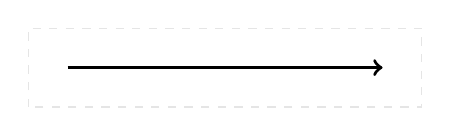
\begin{tikzpicture}
                \draw[dashed,white!90!black] (0,0) rectangle (5,1);
                \draw[very thick,->] (0.5,0.5) -- ++ (0:4cm);
            \end{tikzpicture}
        }
    \end{choices}
\end{question}
}

\element{project}{
\begin{question}{testB-Q11}
    Gravitational and electrostatic (coulomb) forces are similar in many ways but differ in others.
    Which one of the following statements is \emph{not} true for both gravitational and electrostatic forces?
    \begin{choices}
        \wrongchoice{The force varies at $\dfrac{1}{R^2}$.}
        \wrongchoice{The force depends upon the quantity (mass or charge) on which the force acts.}
      \correctchoice{The force can be attractive and repulsive.}
        \wrongchoice{The force law can be tested in the laboratory.}
    \end{choices}
\end{question}
}

\element{project}{
\begin{question}{testB-Q12}
    The Angstrom (\si{\angstrom}) is a unit of:
    \begin{multicols}{2}
    \begin{choices}
        \wrongchoice{mass.}
        \wrongchoice{time.}
        \wrongchoice{speed.}
      \correctchoice{length.}
    \end{choices}
    \end{multicols}
\end{question}
}

%% NOTE: duplicate of testA-Q09
\element{project}{
\begin{questionmult}{testB-Q13}
    The direction of the electric field in a plane electromagnetic wave is:
    \begin{choices}
        \wrongchoice{perpendicular to the magnetic field and in the direction of the wave's propagation.}
      \correctchoice{perpendicular to the magnetic field and perpendicular to the direction of the wave's propagation.}
        \wrongchoice{parallel to the magnetic field. }
    \end{choices}
\end{questionmult}
}

\element{project}{
\begin{question}{testB-Q14}
    The wavelength of visible light is most nearly the same as:
    \begin{choices}
        \wrongchoice{the length of a football field.}
        \wrongchoice{your height.}
        \wrongchoice{the diameter of an apple.}
        \wrongchoice{the diameter of a pencil.}
      \correctchoice{the thickness of a soap bubble.}
    \end{choices}
\end{question}
}

\element{project}{
\begin{question}{testB-Q15}
    A conclusion that could be drawn from the experiment of Michelson and Morley was that:
    \begin{choices}
        \wrongchoice{the speed of light is greater in a vacuum than in glass.}
        \wrongchoice{light is an electromagnetic radiation.}
        \wrongchoice{the earth moves through the ether.}
        \wrongchoice{light consists of particles, not waves.}
      \correctchoice{there is no ether.}
    \end{choices}
\end{question}
}


%% Test C
%%--------------------
\element{project}{
\begin{question}{testC-Q01}
    A unit of electric potential difference is the:
    \begin{multicols}{2}
    \begin{choices}
        \wrongchoice{ampere (\si{\ampere}).}
        \wrongchoice{ohm (\si{\ohm}).}
      \correctchoice{volt (\si{\volt}).}
        \wrongchoice{joule (\si{\joule}).}
        \wrongchoice{coulomb (\si{\coulomb}).}
    \end{choices}
    \end{multicols}
\end{question}
}

\element{project}{
\begin{question}{testC-Q02}
    Arrange the following units of length in
        order of increasing magnitude.
    \begin{enumerate}
        \itemsep=0pt
        \item centimeter  (\si{\centi\meter})
        \item angstrom  (\si{\angstrom})
        \item meter  (\si{\meter})
    \end{enumerate}
    The correct arrangement is:
    \begin{multicols}{2}
    \begin{choices}
        \wrongchoice{1, 2, 3.}
        \wrongchoice{2, 3, 1.}
        \wrongchoice{3, 1, 2.}
      \correctchoice{2, 1, 3.}
        \wrongchoice{3, 2, 1.}
        %% NOTE: add one to make even
        \wrongchoice{1, 3, 2.}
    \end{choices}
    \end{multicols}
\end{question}
}

\element{project}{
\begin{question}{testC-Q03}
    The equations that led to the prediction that light is an
        electromagnetic phenomenon were derived by:
    \begin{choices}
        \wrongchoice{Charles-Augustin de Coulomb.}
        \wrongchoice{Hans Christian {\o}rsted.}
        \wrongchoice{Michael Faraday.}
      \correctchoice{Jame Clerk Maxwell.}
        \wrongchoice{Andr\'{e}-Marie Amp\`{e}re.}
    \end{choices}
\end{question}
}

%% NOTE: duplicate of testB-Q02
\element{project}{
\begin{question}{testC-Q04}
    \emph{All except one} of the following satisfy the
        definition of a field as given in the text.
    Find the exception.
    \begin{choices}
        \wrongchoice{water temperature in Lake Michigan}
        \wrongchoice{density of smoke in the air above New York}
        \wrongchoice{noise level in a stadium during a baseball game}
        \wrongchoice{depth of snow on the ground during a blizzard}
      \correctchoice{the total number of babies born in the United States during 1965}
    \end{choices}
\end{question}
}

\element{project}{
\begin{question}{testC-Q05}
    Which one of the following statements is correct?
    \begin{choices}
        \wrongchoice{Electricity and magnetism are unrelated phenomena.}
        \wrongchoice{Magnets can produce electric currents, but electric currents cannot produce magnetic fields.}
      \correctchoice{Magnets can produce electric currents and electric currents can produce magnetic fields.}
        \wrongchoice{Electric currents cannot produce magnetic fields.}
        \wrongchoice{Electricity and magnetism are identical properties of lodestones.}
    \end{choices}
\end{question}
}

\element{project}{
\begin{question}{testC-Q06}
    Two uncharged conducting spheres are suspended
        by nylon threads and touch each other.
    \begin{center}
    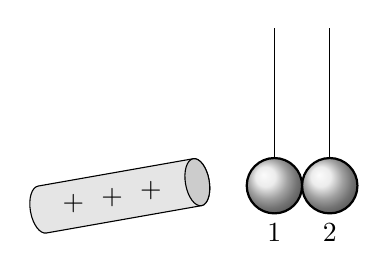
\begin{tikzpicture}
        %% Two spheres
        \draw (-1em,0) -- ++(90:2);
        \draw (+1em,0) -- ++(90:2);
        \draw[thick,shading=ball,ball color=white!90!black] (-1em,0) circle (1em) node[anchor=north,yshift=-1em] {1};
        \draw[thick,shading=ball,ball color=white!90!black] (+1em,0) circle (1em) node[anchor=north,yshift=-1em] {2};
        %% charged bar
        \begin{scope}[xshift=-3.3cm,yshift=-2ex,rotate=10]
            \draw[fill=white!90!black] (0,2ex) -- (2,2ex) arc (90:-90:1ex and 2ex) -- (0,-2ex) arc (270:90:1ex and 2ex);
            \draw[fill=white!80!black] (2,2ex) arc (90:270:1ex and 2ex) arc (-90:90:1ex and 2ex);
            \node[anchor=center] at (0.4,0) {$+$};
            \node[anchor=center] at (0.9,0) {$+$};
            \node[anchor=center] at (1.4,0) {$+$};
        \end{scope}
    \end{tikzpicture}
    \end{center}
    With a positively charged rod held \emph{near} sphere 1 the two spheres separate.
    The charges on the two spheres will be:
    \begin{choices}
        %% \makebox[width][position]{text}
        %% NOTE: Charging an object by induction
        \wrongchoice{\makebox[6em][l]{1: none,}     \makebox[6em][l]{2: positive}}
      \correctchoice{\makebox[6em][l]{1: negative,} \makebox[6em][l]{2: positive}}
        \wrongchoice{\makebox[6em][l]{1: none,}     \makebox[6em][l]{2: none}}
        \wrongchoice{\makebox[6em][l]{1: negative,} \makebox[6em][l]{2: none}}
    \end{choices}
\end{question}
}

\element{project}{
\begin{questionmult}{testC-Q07}
    The electric field vector at a point in an electrostatic field indicates:
    \begin{choices}
      \correctchoice{the magnitude of the electrostatic force exerted per unit charge at that point.}
      \correctchoice{the direction of the electrostatic force exerted per unit charge at that point.}
        \wrongchoice{the electric charge at that point.}
    \end{choices}
\end{questionmult}
}

%% NOTE: duplicate of testA-Q03
\element{project}{
\begin{question}{testC-Q08}
    A narrow beam of light emerges from a block of ordinary
        glass in the direction shown in the diagram.
    Which arrow in the diagram best represents the path
        of the beam within the glass?
    \begin{center}
    \begin{tikzpicture}
        %% NOTE: used n=1.50 for glass
        %% glass
        \draw[white,fill=white!90!black] (0,-2) arc(270:90:2) -- cycle;
        %% surface
        \draw[line width=1pt] (0,-2.1) -- (0,2.1);
        %% incoming
        \foreach \a/\b in {120/A,135/B,150/C,180/D,200/E} {
            \draw[thick,postaction={decorate},decoration={markings, mark=at position 0.5 with {\arrow{latex}}}] (\a:2.33) -- (0,0) node[pos=0,anchor=center,shift={(\a:1em)}] {$\b$};
        }
        %% outgoing
        \draw[thick,->] (0,0) -- (315:2);
        %% labels
        \node[anchor=north] at (-0.8,-2.2) {glass};
        \node[anchor=north] at (+0.8,-2.2) {air};
    \end{tikzpicture}
    \end{center}
    \begin{multicols}{5}
    \begin{choices}[o]
        \wrongchoice{$A$}
        \wrongchoice{$B$}
      \correctchoice{$C$}
        \wrongchoice{$D$}
        \wrongchoice{$E$}
    \end{choices}
    \end{multicols}
\end{question}
}

\element{project}{
\begin{question}{testC-Q09}
    Newton's synthesis of terrestrial and celestial mechanics
        incorporated the work of Kepler and Galileo.
    In a similar way, the work of {\o}rsted and Faraday
        was incorporated in the synthesis made by:
    %Hans Christian Ørsted
    %Michael Faraday
    \begin{choices}
        \wrongchoice{Andr\'{e}-Marie Amp\`{e}re.}
        \wrongchoice{Heinrich Rudolf Hertz.}
      \correctchoice{James Clerk Maxwell.}
        \wrongchoice{William Gilbert.}
    \end{choices}
\end{question}
}

\element{project}{
\begin{question}{testC-Q10}
    A glass prism separates white light into the colors of the spectrum because:
    \begin{choices}
        \wrongchoice{light is reflected inside the prism.}
      \correctchoice{different frequencies of light move with different speeds in the prism.}
        \wrongchoice{different frequencies of light superpose in the prism.}
        \wrongchoice{electromagnetic energy is dissipated inside the prism.}
    \end{choices}
\end{question}
}

%% NOTE: duplicate of testB-Q01
\element{project}{
\begin{question}{testC-Q11}
    Which of the following graphs best represents the way the
        force one small charged body exerts on another changes
        when the distance between their centers is changed?
    \begin{multicols}{2}
    \begin{choices}
        \AMCboxDimensions{down=-2.5em}
        \wrongchoice{
            \begin{tikzpicture}
                \begin{axis}[
                    axis y line=left,
                    axis x line=bottom,
                    axis line style={->},
                    xlabel={distance},
                    xtick=\empty,
                    ylabel={force},
                    ytick=\empty,
                    xmin=0,xmax=11,
                    ymin=0,ymax=11,
                    width=1.00\columnwidth,
                    very thin,
                ]
                \addplot[line width=1pt,domain=0:10]{8};
                \end{axis}
            \end{tikzpicture}
        }
        \wrongchoice{
            \begin{tikzpicture}
                \begin{axis}[
                    axis y line=left,
                    axis x line=bottom,
                    axis line style={->},
                    xlabel={distance},
                    xtick=\empty,
                    ylabel={force},
                    ytick=\empty,
                    xmin=0,xmax=11,
                    ymin=0,ymax=11,
                    width=1.00\columnwidth,
                    very thin,
                ]
                \addplot[line width=1pt,domain=0:10]{x};
                \end{axis}
            \end{tikzpicture}
        }
        \wrongchoice{
            \begin{tikzpicture}
                \begin{axis}[
                    axis y line=left,
                    axis x line=bottom,
                    axis line style={->},
                    xlabel={distance},
                    xtick=\empty,
                    ylabel={force},
                    ytick=\empty,
                    xmin=0,xmax=11,
                    ymin=0,ymax=11,
                    width=1.00\columnwidth,
                    very thin,
                ]
                \addplot[line width=1pt,domain=0:10]{10-x};
                \end{axis}
            \end{tikzpicture}
        }
        \wrongchoice{
            \begin{tikzpicture}
                \begin{axis}[
                    axis y line=left,
                    axis x line=bottom,
                    axis line style={->},
                    xlabel={distance},
                    xtick=\empty,
                    ylabel={force},
                    ytick=\empty,
                    xmin=0,xmax=11,
                    ymin=0,ymax=11,
                    width=1.00\columnwidth,
                    very thin,
                ]
                \addplot[line width=1pt,domain=0:10]{0.1*x*x};
                \end{axis}
            \end{tikzpicture}
        }
        %% NOTE: F = gmm/R^2
        %% NOTE: should be 10/x/x, but this is easier to see
        \correctchoice{
            \begin{tikzpicture}
                \begin{axis}[
                    axis y line=left,
                    axis x line=bottom,
                    axis line style={->},
                    xlabel={distance},
                    xtick=\empty,
                    ylabel={force},
                    ytick=\empty,
                    xmin=0,xmax=11,
                    ymin=0,ymax=11,
                    width=1.00\columnwidth,
                    very thin,
                ]
                \addplot[line width=1pt,domain=0:10]{10/x};
                \end{axis}
            \end{tikzpicture}
        }
    \end{choices}
    \end{multicols}
\end{question}
}

\element{project}{
\begin{question}{testC-Q12}
    Which of the following graphs best represents the force
        on a charged particle moving across a uniform magnetic field
        when the particle's speed increases?
    \begin{multicols}{2}
    \begin{choices}
        \AMCboxDimensions{down=-2.5em}
        \wrongchoice{
            \begin{tikzpicture}
                \begin{axis}[
                    axis y line=left,
                    axis x line=bottom,
                    axis line style={->},
                    xlabel={speed},
                    xtick=\empty,
                    ylabel={force},
                    ytick=\empty,
                    xmin=0,xmax=11,
                    ymin=0,ymax=11,
                    width=1.00\columnwidth,
                    very thin,
                ]
                \addplot[line width=1pt,domain=0:10]{8};
                \end{axis}
            \end{tikzpicture}
        }
        %% NOTE: F = qvB
        \correctchoice{
            \begin{tikzpicture}
                \begin{axis}[
                    axis y line=left,
                    axis x line=bottom,
                    axis line style={->},
                    xlabel={speed},
                    xtick=\empty,
                    ylabel={force},
                    ytick=\empty,
                    xmin=0,xmax=11,
                    ymin=0,ymax=11,
                    width=1.00\columnwidth,
                    very thin,
                ]
                \addplot[line width=1pt,domain=0:10]{x};
                \end{axis}
            \end{tikzpicture}
        }
        \wrongchoice{
            \begin{tikzpicture}
                \begin{axis}[
                    axis y line=left,
                    axis x line=bottom,
                    axis line style={->},
                    xlabel={speed},
                    xtick=\empty,
                    ylabel={force},
                    ytick=\empty,
                    xmin=0,xmax=11,
                    ymin=0,ymax=11,
                    width=1.00\columnwidth,
                    very thin,
                ]
                \addplot[line width=1pt,domain=0:10]{10-x};
                \end{axis}
            \end{tikzpicture}
        }
        \wrongchoice{
            \begin{tikzpicture}
                \begin{axis}[
                    axis y line=left,
                    axis x line=bottom,
                    axis line style={->},
                    xlabel={speed},
                    xtick=\empty,
                    ylabel={force},
                    ytick=\empty,
                    xmin=0,xmax=11,
                    ymin=0,ymax=11,
                    width=1.00\columnwidth,
                    very thin,
                ]
                \addplot[line width=1pt,domain=0:10]{0.1*x*x};
                \end{axis}
            \end{tikzpicture}
        }
        \wrongchoice{
            \begin{tikzpicture}
                \begin{axis}[
                    axis y line=left,
                    axis x line=bottom,
                    axis line style={->},
                    xlabel={speed},
                    xtick=\empty,
                    ylabel={force},
                    ytick=\empty,
                    xmin=0,xmax=11,
                    ymin=0,ymax=11,
                    width=1.00\columnwidth,
                    very thin,
                ]
                \addplot[line width=1pt,domain=0:10]{10/x};
                \end{axis}
            \end{tikzpicture}
        }
    \end{choices}
    \end{multicols}
\end{question}
}

%% NOTE: duplicate of testB-Q15
%% NOTE: trivial rewording
\element{project}{
\begin{question}{testC-Q13}
    A conclusion drawn from the experiment of Michelson and Morley was that:
    \begin{choices}
        \wrongchoice{the speed of light is greater in a vacuum than in glass.}
        \wrongchoice{light is an electromagnetic radiation.}
        \wrongchoice{the earth moves through the ether with the speed of light.}
        \wrongchoice{light consists of particles, not waves.}
      \correctchoice{there is no ether.}
    \end{choices}
\end{question}
}

%% NOTE: duplicate of testB-Q03
\element{project}{
\begin{question}{testC-Q14}
    Which of the following is \emph{not} an electromagnetic wave phenomenon?
    \begin{choices}
        \wrongchoice{radar}
        \wrongchoice{ultraviolet light}
      \correctchoice{sound}
        \wrongchoice{x-radiation}
    \end{choices}
\end{question}
}

\element{project}{
\begin{questionmult}{testC-Q15}
    Which of the following produce(s) a magnetic field?
    \begin{choices}
      \correctchoice{an electric current in a wire}
      \correctchoice{a moving charged particle}
      \correctchoice{a changing electric field}
    \end{choices}
\end{questionmult}
}

%% NOTE: duplicate of testA-Q07 and testB-Q08
\element{project}{
\begin{question}{testC-Q16}
    In a vacuum, electromagnetic radiations, such as radio waves,
        light, x rays and gamma rays have the same:
    \begin{choices}
        \wrongchoice{wavelength.}
        \wrongchoice{frequency.}
        \wrongchoice{period.}
      \correctchoice{speed.}
        \wrongchoice{amplitude.}
    \end{choices}
\end{question}
}

\element{project}{
\begin{question}{testC-Q17}
    $P$ watts of power are dissipated in the form of heat when
        a current $I$ flows through a heater coil whose resistance is $R$.
    If the current through the coil is doubled,
        how much power will be dissipated in the form of heat?
    \begin{multicols}{2}
    \begin{choices}
        \wrongchoice{$\dfrac{1}{4}P$ watts}
        \wrongchoice{$\dfrac{1}{2}P$ watts}
        \wrongchoice{$P$ watts}
      \correctchoice{$2P$ watts}
        \wrongchoice{$4P$ watts}
    \end{choices}
    \end{multicols}
\end{question}
}

%% NOTE: duplicate of testB-Q11
\element{project}{
\begin{question}{testC-Q18}
    Gravitational and electrostatic (Coulomb) forces are
        similar in many ways but differ in others.
    Which one of the following statements is \emph{not} true for
        both gravitational and electrostatic forces?
    \begin{choices}
        \wrongchoice{The force varies as $\dfrac{1}{R^2}$.}
        \wrongchoice{The force depends upon the quantity (mass or charge) on which the force acts.}
      \correctchoice{The force can be attractive and repulsive.}
        \wrongchoice{The force law can be tested in the laboratory.}
    \end{choices}
\end{question}
}

%% NOTE: duplicate of testA-Q09 and testB-Q13
\element{project}{
\begin{questionmult}{testC-Q19}
    The direction of the electric field in a plane electromagnetic wave is:
    \begin{choices}
        \wrongchoice{perpendicular to the magnetic field and perpendicular to the direction of the wave's propagation.}
      \correctchoice{perpendicular to the magnetic field and in the direction of the wave's propagation.}
        \wrongchoice{parallel to the magnetic field.}
    \end{choices}
\end{questionmult}
}

%\element{project}{
%\begin{question}{testC-Q20}
%    A wire carrying a large and constant electric current passes
%        through the center of and perpendicular to a piece of cardboard,
%        as shown at right.
%    If iron filings are sprinkled on the cardboard,
%        how will they arrange themselves?
%    %% NOTE: TODO: tikz, complex
%    \begin{choices}
%        \wrongchoice{
%            \begin{tikzpicture}
%            \end{tikzpicture}
%        }
%    \end{choices}
%\end{question}
%}

%% NOTE: duplicate of testA-Q01
\element{project}{
\begin{question}{testC-Q21}
    A person whose eyes are located at point $P$ is looking into the mirror.
    \begin{center}
    \begin{tikzpicture}
        %% mirror
        \draw[line width=1pt] (-0.15,0) -- (2.15,0) node[pos=0.5,anchor=south] {mirror};
        %% point P
        \draw[fill] (-1.5,-0.5) circle (1.5pt) node[anchor=east] {$P$};
        %% cards 1,2,3,4
        \node[draw,minimum height=1.5em,minimum width=0.5em,anchor=north] at (0,-0.25) {1};
        \node[draw,minimum height=1.5em,minimum width=0.5em,anchor=north] at (2,-0.25) {2};
        \node[draw,minimum height=1.5em,minimum width=0.5em,anchor=north] at (1,-2) {4};
        \node[draw,minimum height=1.5em,minimum width=0.5em,anchor=north] at (4,-0.25) {3};
    \end{tikzpicture}
    \end{center}
    Which of the numbered cards can he see reflected in the mirror?
    %% NOTE: questionmult?
    \begin{choices}
        \wrongchoice{1 and 4}
      \correctchoice{2 and 3}
        \wrongchoice{1, 2 and 3}
        \wrongchoice{1, 2, 3 and 4}
    \end{choices}
\end{question}
}

\element{project}{
\begin{question}{testC-Q22}
    The wave and particle models of light predict contradictory
        values of the velocity of light when used to explain:
    \begin{choices}
        \wrongchoice{reflection of light.}
        %% Particle model predicts an increase in speed
      \correctchoice{refraction of light.}
        \wrongchoice{polarization.}
        \wrongchoice{superposition.}
    \end{choices}
\end{question}
}

\element{project}{
\begin{questionmult}{testC-Q23}
    %Consider the following situations.
    In which of the below is a current produced in the wire loop?
    \begin{choices}
        \wrongchoice{a wire loop surrounding a wire with a steady current.}
      \correctchoice{a magnet dropping through a wire loop.}
        \wrongchoice{a stationary charged sphere at the center of a wire loop.}
    \end{choices}
\end{questionmult}
}

\element{project}{
\begin{question}{testC-Q24}
    Which of the following is the chief physical principle
        on which the operation of an electric generator depends?
    \begin{choices}
      \correctchoice{A current is induced in a wire moving through a magnetic field.}
        \wrongchoice{The electric field strength varies as the inverse square of the distance from a charge.}
        \wrongchoice{Two current-carrying wires exert forces on one another.}
        \wrongchoice{An alternating current produces electromagnetic radiation.}
    \end{choices}
\end{question}
}

%% NOTE: duplicate of testB-Q12
\element{project}{
\begin{question}{testC-Q25}
    The Angstrom (\si{\angstrom}) is a unit of:
    \begin{multicols}{2}
    \begin{choices}
        \wrongchoice{mass}
        \wrongchoice{time}
        \wrongchoice{speed}
      \correctchoice{length}
    \end{choices}
    \end{multicols}
\end{question}
}

\element{project}{
\begin{question}{testC-Q26}
    Which of the following could you measure to find your true motion through space?
    \begin{choices}
        \wrongchoice{apparent speed of light}
        \wrongchoice{speed of the motion relative to the ether}
        \wrongchoice{speed of the motion relative to some stationary object}
        %% NOTE: consider questionmult with all answers as wrong
      \correctchoice{none of the provided}
    \end{choices}
\end{question}
}

\element{project}{
\begin{question}{testC-Q27}
    A vertical wire hidden in a wall is carrying a direct current.
    What piece of equipment might help you find the location of the wire?
    \begin{multicols}{2}
    \begin{choices}
        \wrongchoice{transformer}
        \wrongchoice{dc generator}
      \correctchoice{compass}
        \wrongchoice{radio receiver}
    \end{choices}
    \end{multicols}
\end{question}
}

\element{project}{
\begin{question}{testC-Q28}
    Two identically charged small spheres are at a distance $r$ meters apart.
    If the distance is doubled to $2r$ meters,
        the force exerted on each sphere will:
    \begin{choices}
        \wrongchoice{change to $4$ times the original value.}
        \wrongchoice{change to $2$ times the original value.}
        \wrongchoice{not change.}
        \wrongchoice{change to $\dfrac{1}{2}$ the original value.}
      \correctchoice{change to $\dfrac{1}{4}$ the original value.}
    \end{choices}
\end{question}
}

%\element{project}{
%\begin{question}{testC-Q29}
%    In the apparatus shown at right,
%        a beam of positively charged particles is directed horizontally
%        into the field between two magnets.
%    What is the effect of the magnetic field?
%    \begin{center}
%    \begin{tikzpicture}
%        %% NOTE: TODO: tikz picture, complex
%    \end{tikzpicture}
%    \end{center}
%    \begin{choices}
%        \wrongchoice{The particles continue in the same direction with the same speed.}
%        \wrongchoice{The particles are accelerated toward the S magnetic pole.}
%        \wrongchoice{The particles are accelerated toward the N magnetic pole.}
%        \wrongchoice{The particles are accelerated upward.}
%        %% NOTE: needed to add the correct option
%        \wrongchoice{The particles are accelerated downward.}
%    \end{choices}
%\end{question}
%}

%% NOTE: near duplicate of testB-Q05
\element{project}{
\begin{question}{testC-Q30}
    Questions 30, 31 and 32 list the names of scientists who made
        significant contributions in the study of light.
    Select the statement from the list below that best describes
        the scientific contribution of Thomas Young.
    \begin{choices}
      \correctchoice{Light exhibits the phenomenon of interference.}
        \wrongchoice{Color is not an inherent property of an object,
            but depends on how the object reflects and absorbs the various colored rays that strike it.}
        \wrongchoice{Invented a plastic sheet that would polarize light.}
        \wrongchoice{Developed a mathematical wave theory of light.}
    \end{choices}
\end{question}
}

%% NOTE: near duplicate of testB-Q06
\element{project}{
\begin{question}{testC-Q31}
    Select the statement from the list below that best describes
        the scientific contribution of Augustin-Jean Fresnel.
    \begin{choices}
        \wrongchoice{Light exhibits the phenomenon of interference.}
        \wrongchoice{Color is not an inherent property of an object,
            but depends on how the object reflects and absorbs the various colored rays that strike it.}
        \wrongchoice{Invented a plastic sheet that would polarize light.}
      \correctchoice{Developed a mathematical wave theory of light.}
    \end{choices}
\end{question}
}

\element{project}{
\begin{question}{testC-Q32}
    Select the statement from the list below that best describes
        the scientific contribution of Isaac Newton.
    \begin{choices}
        \wrongchoice{Light exhibits the phenomenon of interference.}
      \correctchoice{Color is not an inherent property of an object,
            but depends on how the object reflects and absorbs the various colored rays that strike it.}
        \wrongchoice{Invented a plastic sheet that would polarize light.}
        \wrongchoice{Developed a mathematical wave theory of light.}
    \end{choices}
\end{question}
}

\element{project}{
\begin{question}{testC-Q33}
    Three identical metal balls $A$, $B$, and $C$ are mounted on insulating rods.
    Ball $A$ has a charge $+q$, while balls $B$ and $C$ are uncharged.
    Ball $A$ is brought into contact momentarily with ball $B$, and then with ball $C$.
    At the end of this experiment, the charge on ball $A$ will be:
    \begin{choices}
        \wrongchoice{$+q$.}
        \wrongchoice{$+\dfrac{q}{2}$.}
        \wrongchoice{$+\dfrac{q}{3}$.}
      \correctchoice{$+\dfrac{q}{4}$.}
        \wrongchoice{No charge remains on $A$.}
    \end{choices}
\end{question}
}

%% NOTE: duplicate of testA-Q13
\element{project}{
\begin{question}{testC-Q34}
    Select the statement that best describes the scientific contribution of James Clerk Maxwell.
    \begin{choices}
        \wrongchoice{Two current-carrying wires exert forces on each other.}
      \correctchoice{An electric field changing with time generates a magnetic field.}
        \wrongchoice{An electric current exerts a force on a magnet.}
        \wrongchoice{A magnetic field changing with time can cause a current to flow in a wire.}
    \end{choices}
\end{question}
}

%% NOTE: duplicate of testA-Q14
\element{project}{
\begin{question}{testC-Q35}
    Select the statement that best describes the scientific contribution of Andr\'{e}-Marie Amp\`{e}re.
    \begin{choices}
      \correctchoice{Two current-carrying wires exert forces on each other.}
        \wrongchoice{An electric field changing with time generates a magnetic field.}
        \wrongchoice{An electric current exerts a force on a magnet.}
        \wrongchoice{A magnetic field changing with time can cause a current to flow in a wire.}
    \end{choices}
\end{question}
}

%% NOTE: duplicate of testA-Q15
\element{project}{
\begin{question}{testC-Q36}
    Select the statement that best describes the scientific contribution of Michael Faraday.
    \begin{choices}
        \wrongchoice{Two current-carrying wires exert forces on each other.}
        \wrongchoice{An electric field changing with time generates a magnetic field.}
        \wrongchoice{An electric current exerts a force on a magnet.}
      \correctchoice{A magnetic field changing with time can cause a current to flow in a wire.}
    \end{choices}
\end{question}
}

\element{project}{
\begin{question}{testC-Q37}
    An electric motor that draws \SI{2}{\ampere} of current when
        operating at \SI{110}{\volt} can do work at the rate of:
    \begin{multicols}{2}
    \begin{choices}
        \wrongchoice{\SI{55}{\watt}}
        \wrongchoice{\SI{110}{\watt}}
      \correctchoice{\SI{220}{\watt}}
        \wrongchoice{\SI{440}{\watt}}
    \end{choices}
    \end{multicols}
\end{question}
}

\element{project}{
\begin{question}{testC-Q38}
    Which one of the following scientists first demonstrated
        experimentally that the earth behaves like a large magnet?
    \begin{choices}
        %% NOTE: added first name also
        \wrongchoice{William Gilbert.}
      \correctchoice{Hans Christian {\o}rsted.}
        \wrongchoice{Michael Faraday}
        \wrongchoice{James Clerk Maxwell}
        \wrongchoice{Andr\'{e}-Marie Amp\`{e}re.}
    \end{choices}
\end{question}
}

\element{project}{
\begin{questionmult}{testC-Q39}
    A charged particle moves through a uniform magnetic field.
    The effect of the field can change the particle's:
    \begin{choices}
      \correctchoice{velocity.}
        \wrongchoice{speed.}
        \wrongchoice{energy.}
    \end{choices}
\end{questionmult}
}

%% NOTE: duplicate of testA-Q11
\element{project}{
\begin{question}{testC-Q40}
    A transformer can be used to change:
    \begin{choices}
        \wrongchoice{electrical energy into mechanical energy.}
        \wrongchoice{mechanical energy into electrical energy.}
        \wrongchoice{high voltage dc to low voltage dc.}
      \correctchoice{low voltage ac to high voltage ac.}
    \end{choices}
\end{question}
}

\endinput

